% Tamaño de letra.
\documentclass[12pt,titlepage]{article}

%------------------------------ Paquetes ----------------------------------

% Paquetes:

%Para comentarios multilínea.
\usepackage{verbatim}

% Para tener cabecera y pie de página con un estilo personalizado.
\usepackage{fancyhdr}

% Codificación UTF-8
\usepackage[utf8]{inputenc}

% Castellano.
\usepackage[spanish]{babel}

% Tamaño de página y márgenes.
\usepackage[a4paper,headheight=16pt,scale={0.75,0.8},hoffset=0.5cm]{geometry}


% Para poder agregar notas al pie en tablas:
%\usepackage{threeparttable}

% Tipo de letra Helvetica (Arial).
%\usepackage{helvet}
%\renewcommand\familydefault{\sfdefault}

% Gráficos:

% Para incluir imágenes, el siguiente código carga el paquete graphicx
% según se esté generando un archivo dvi o un pdf (con pdflatex).

% Para generar dv.
%\usepackage[dvips]{graphicx}

% Para generar pdf.
\usepackage[pdftex]{graphicx}
\pdfcompresslevel=9

\usepackage{pdfpages}

% Para códigos fuente.
\usepackage{listings}

% Para links.
%\usepackage{hyperref}

\usepackage[section]{placeins}

\usepackage{appendix}
\usepackage{ulem}
\usepackage{float}


%
% Directorio donde están las imagenes.
%
%\newcommand{\imgdir}{includes}
%\graphicspath{{\imgdir/}}

%------------------------------ ~paquetes ---------------------------------

%------------------------- Inicio del documento ---------------------------

\begin{document}

% ---------------------- Encabezado y pie de página -----------------------

% Encabezado: sección a la derecha.
% Pie de página: número de página a la derecha.

\pagestyle{fancy}
\renewcommand{\sectionmark}[1]{\markboth{}{\thesection\ \ #1}}
\lhead{}
\chead{}
\rhead{\rightmark}
\lfoot{}
\cfoot{}
\rfoot{\thepage}

% ---------------------- ~Encabezado y pie de página ----------------------

% -------------------------- Título y autor(es) ---------------------------

\title{???}
\author{}

% -------------------------- ~Título y autor(es) --------------------------

% ------------------------------- Carátula --------------------------------

\begin{titlepage}

\thispagestyle{empty}

% Logo facultad más pie de la figura.
\begin{center}

\includegraphics[scale=0.55]{./logo_caratula}\\
\large{\textsc{Universidad de Buenos Aires}}\\
\large{\textsc{Facultad De Ingeniería}}\\
\small{Año 2011 - 1\textsuperscript{er} Cuatrimestre}
\end{center}

\vfill

% Título central.
\begin{center}

\Large{\underline{\textsc{Introducción a los Sistemas Distribuidos (75.43)}}}

\vfill

% Tabla de integrantes.

\Large{\underline{\textsc{Trabajo Práctico Grupal}}}

\vfill

\Large\underline{Integrantes} \linebreak\linebreak

% Separación entre columnas.
\large\addtolength{\tabcolsep}{-3pt}
% Tres columnas con alineación centrada.
\begin{tabular}{|| c | c | c ||}
  \hline
    \textbf{Apellido, Nombre} & \textbf{Nro. Padrón} & \textbf{E-mail} \\
  \hline
    Mari, Sebastian & XXXX & XXXX@gmail.com \\
  \hline
    Morandi, Nicolas & XXXX & XXXX@gmail.com \\
  \hline
    Piccoli, Sebastian & XXXX & seba.piccoli@gmail.com \\
  \hline
    Roberts, Karen & 88062 & karenroberts16@gmail.com \\
  \hline
    Wolsdorf, Diego & XXXX & XXXX@gmail.com \\
  \hline
    Ygounet, Guido & 88246 & gygounet@gmail.com \\
  \hline
\end{tabular}
\end{center}

\vfill

\hrule
\vspace{0.2cm}

% Pie de página de la carátula.
\noindent\small{75.43 - Introduccion a los Sistemas Distribuidos}

\end{titlepage}

% ------------------------------- ~Carátula -------------------------------

% -------------------------------- Índice ---------------------------------

% Hago que las páginas se comiencen a contar a partir de aquí.
\setcounter{page}{1}

% Índice.
\tableofcontents
\newpage

% -------------------------------- ~Índice --------------------------------

% ----------------------------- Inicio del tp -----------------------------

\section{Determinación de las subredes}

En base a la topolog\'ia propuesta y utilizando la RFC950, se asignaron las siguientes subredes:

\begin{table}
  \begin{center}
    \begin{tabular}{|l|l|l|l|l|}
      \hline
        \bf{Nombre} & \bf{Hosts} & \bf{Bloque} & \bf{Dirección} & \bf{Máscara} \\
      \hline 
	Moscu		& 247 & 256 & 10.42.5.0     & /24 \\
        Tokyo $^{(*)}$      & 204 & 256 & 10.69.5.0     & /24 \\
        Seul               & 114 & 128 & 10.39.25.128  & /25 \\
        Pekin $^{(*)}$     & 103 & 256 & 192.168.15.0  & /24 \\
        Bagdag $^{(*)}$  & 51  & 64  & 10.39.25.0    & /26 \\
        Singapur $^{(*)}$      & 26  & 32  & 10.69.6.128   & /27 \\
        Taipei              & 21  & 32  & 10.69.6.160   & /27 \\
	Bangkok                & 21  & 32  & 10.39.25.64  & /27 \\       
	Beirut                 & 18  & 32  & 10.69.6.224   & /27 \\
	Kuwait                 & 17  & 32  & 10.69.6.192   & /27 \\
        Yakarta                  & 5   & 8   & 10.27.15.192  & /29 \\
        Damasco             & 2   & 4   & 10.27.15.200  & /30 \\
        Jerusalen                 & 2   & 4   & 10.27.15.204  & /30 \\
        Nueva Deli                 & 2   & 4   & 172.51.5.192  & /30 \\
        Kabul                  & 2   & 4   & 172.51.5.196  & /30 \\
        Katmandu               & 2   & 4   & 172.51.5.200  & /30 \\
        Teheran                 & 2   & 4   & 172.51.5.204  & /30 \\
        Ankara                & 2   & 4   & 135.143.5.0   & /30 \\
        Pionyang               & 2   & 4   & 135.143.5.4   & /30 \\ 
    \hline
    \end{tabular} \\
  \end{center}
  \caption{Asignación de direcciones de red.}
\end{table}
\FloatBarrier

(*): Redes asignadas teniendo en cuenta las direcciones IP fijas de los servidores determinadas por el enunciado. \\

\begin{figure}
  \begin{center}
    \advance\leftskip-3cm
    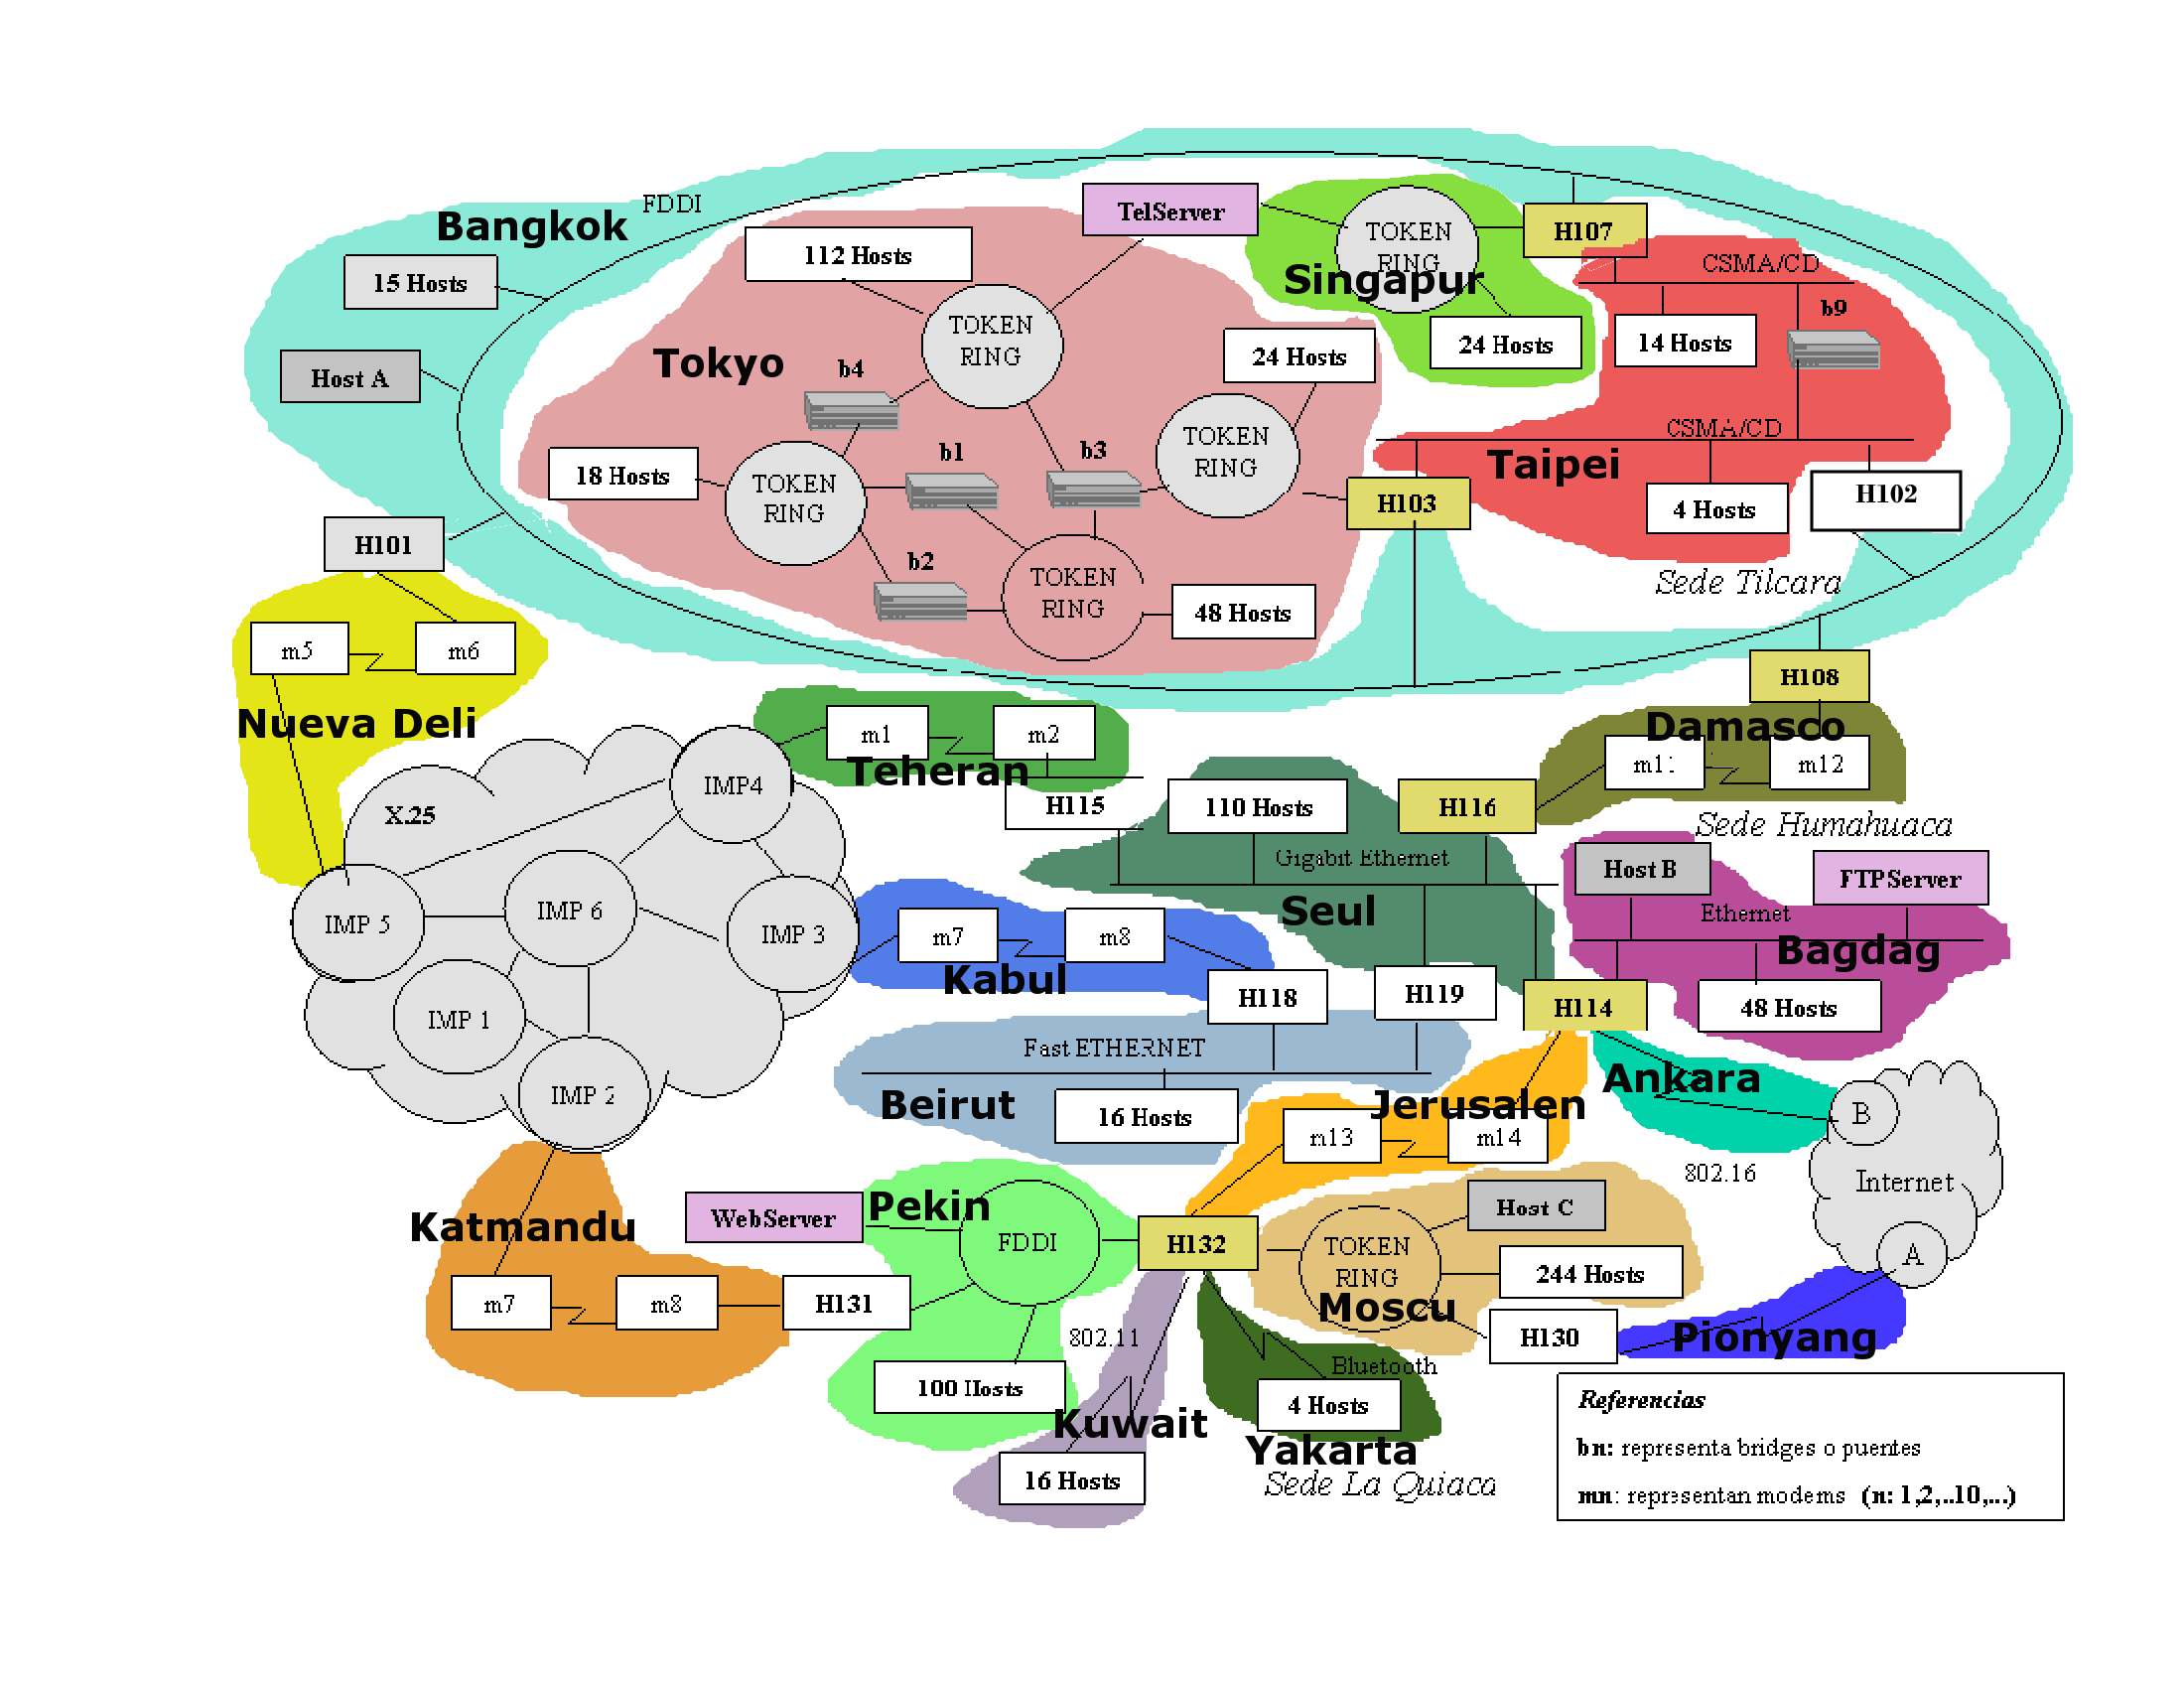
\includegraphics[width=22cm, height=21cm, angle=90]{Subneting.png} \\
  \end{center}
  \caption{Topología de subredes.}
\end{figure}
\FloatBarrier



\section{Tablas de ruteo}


\subsection{Rutas alternativas}




\section{DNS}


\section{Simulación en la sala}

\section{Conclusiones}


% ------------------------------ Bibliografía -------------------------------

\newpage

\begin{thebibliography}{9}

\bibitem{rfc950}
  \emph{RFC 950 - Internet Standard Subnetting Procedure}. \\
  http://www.packetizer.com/rfc/rfc950/

\end{thebibliography}


% ------------------------------ Fin del tp -------------------------------

\end{document}

%---------------------------- Fin del documento ---------------------------
